\documentclass[12pt,a4paper]{article}
\usepackage[utf8]{inputenc}
\usepackage{listings}
\usepackage{graphicx}
\usepackage{hyperref}
\usepackage{url}
\usepackage{float}
\usepackage{color}

\title{1194059 Muhammad Rizal Supriadi 100Error Python}
\author{mrsupriadi2000}
\date{March 2022}

\begin{document}

\maketitle
\thispagestyle{empty}
\newpage
\title{100 Error Pada Python dan Solusinya}
\section{Case Variabel}
\begin{figure}[ht]
    \centerline{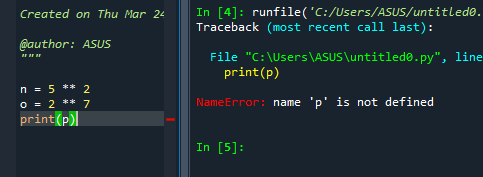
\includegraphics[width=15cm,height=5cm]{image/case1.png}}
    \renewcommand{\figurename}{Gambar}
    \caption{Case-1 Error}
\end{figure}
\paragraph{}\textbf{\textit{Solusi-Case1}} { Mengecek kembali pemanggilan variabel. Berikut merupakan scipt yang benar}
\begin{figure}[ht]
    \centerline{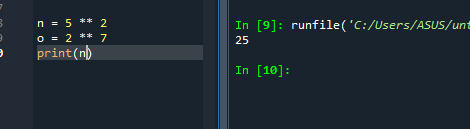
\includegraphics[width=15cm,height=5cm]{image/case1-solved.png}}
    \renewcommand{\figurename}{Gambar}
    \caption{Case-1 Solved}
\end{figure}

% =============================Case 2=============================
\newpage
\section{Case Variabel Value}
\begin{figure}[ht]
    \centerline{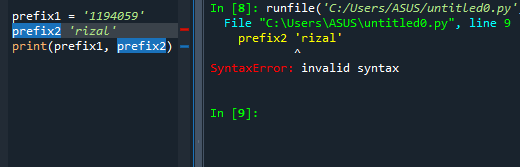
\includegraphics[width=15cm,height=5cm]{image/case2.png}}
    \renewcommand{\figurename}{Gambar}
    \caption{Case-2 Error}
\end{figure}
\paragraph{}\textbf{\textit{Solusi-Case2}} { Mengecek kembali sintax yang ditulis pada bagian prefix2 'rizal' dimana kita lupa menambahkan tanda sama dengan. Berikut merupakan scipt yang benar}
\begin{figure}[ht]
    \centerline{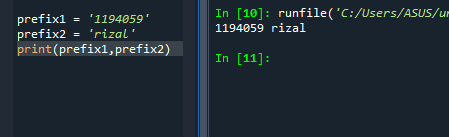
\includegraphics[width=15cm,height=5cm]{image/case2-solved.png}}
    \renewcommand{\figurename}{Gambar}
    \caption{Case-2 Solved}
\end{figure}

% =============================Case 3=============================
\newpage
\section{Case Array}
\begin{figure}[ht]
    \centerline{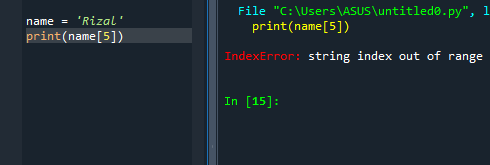
\includegraphics[width=15cm,height=5cm]{image/case3.png}}
    \renewcommand{\figurename}{Gambar}
    \caption{Case-3 Error}
\end{figure}
\paragraph{}\textbf{\textit{Solusi-Case3}} { Menginputkan angka yang bernar pada rentang array 'Rizal' array dimulai dari angka 0, berikut script yang benar}
\begin{figure}[ht]
    \centerline{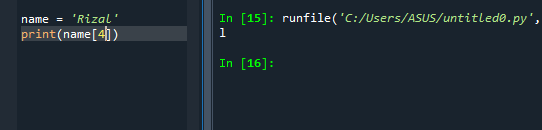
\includegraphics[width=15cm,height=5cm]{image/case3-solved.png}}
    \renewcommand{\figurename}{Gambar}
    \caption{Case-3 Solved}
\end{figure}

% =============================Case 4=============================
\newpage
\section{Case Array}
\begin{figure}[ht]
    \centerline{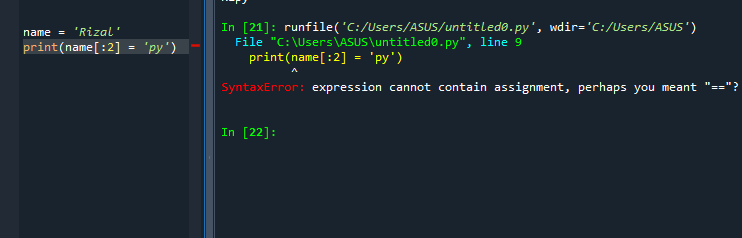
\includegraphics[width=15cm,height=5cm]{image/case4.png}}
    \renewcommand{\figurename}{Gambar}
    \caption{Case-4 Error}
\end{figure}
\paragraph{}\textbf{\textit{Solusi-Case4}} { Dari error diatas kita tau bahwa tanda sama dengan digunakan untuk memasukan nilai ,sedangkan untuk menggaungkan string maka gunakan tanda +}
\begin{figure}[ht]
    \centerline{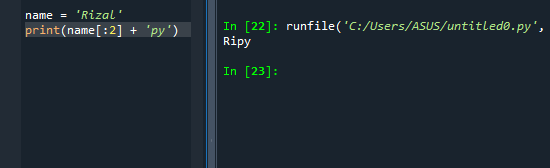
\includegraphics[width=15cm,height=5cm]{image/case4-solved.png}}
    \renewcommand{\figurename}{Gambar}
    \caption{Case-4 Solved}
\end{figure}

% =============================Case 5=============================
\newpage
\section{Case Looping}
\begin{figure}[ht]
    \centerline{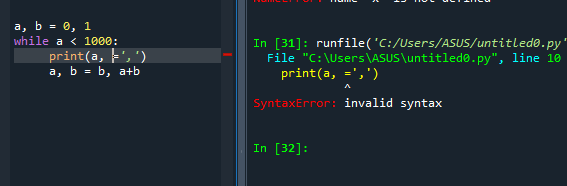
\includegraphics[width=15cm,height=5cm]{image/case5.png}}
    \renewcommand{\figurename}{Gambar}
    \caption{Case-5 Error}
\end{figure}
\paragraph{}\textbf{\textit{Solusi-Case5}} {Pada gambar tersebut menjelaskan error yang terjadi karena sintakx, untuk mengatasiya .. dalam perulangan tersebuat harus menambahkan funsi end di sebelum tanda sama dengan.  }
\begin{figure}[ht]
    \centerline{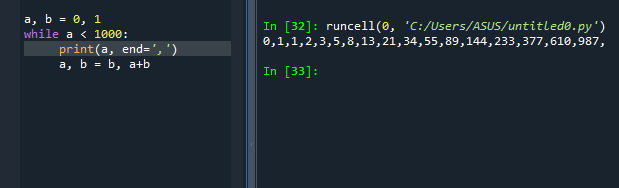
\includegraphics[width=15cm,height=5cm]{image/case5-solved.png}}
    \renewcommand{\figurename}{Gambar}
    \caption{Case-5 Solved}
\end{figure}

% =============================Case 6=============================
\newpage
\section{Case Print}
\begin{figure}[ht]
    \centerline{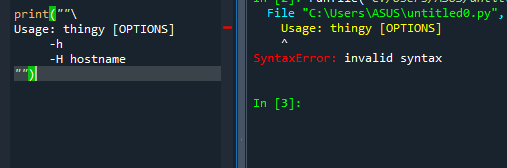
\includegraphics[width=15cm,height=5cm]{image/case6.png}}
    \renewcommand{\figurename}{Gambar}
    \caption{Case-6 Error}
\end{figure}
\paragraph{}\textbf{\textit{Solusi-Case6}} {Ketika kita print beberapa baris secara langsung, maka yang harus dilakukan adalah dengan menggunakan petik 2 .. 3 kali... berikut contoh yang benar}
\begin{figure}[ht]
    \centerline{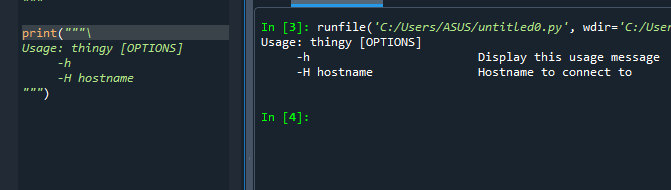
\includegraphics[width=15cm,height=5cm]{image/case6-solved.png}}
    \renewcommand{\figurename}{Gambar}
    \caption{Case-6 Solved}
\end{figure}

% =============================Case 7=============================
\newpage
\section{Case Indentation}
\begin{figure}[ht]
    \centerline{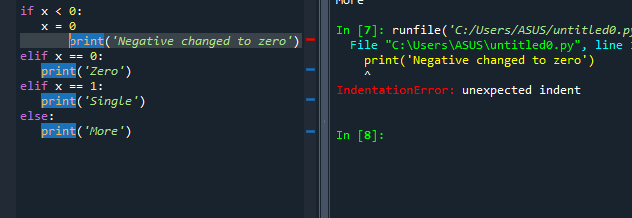
\includegraphics[width=15cm,height=5cm]{image/case7.png}}
    \renewcommand{\figurename}{Gambar}
    \caption{Case-7 Error}
\end{figure}
\paragraph{}\textbf{\textit{Solusi-Case7}} {Error tersebut terjadi karena masalah indentasi, jadi kita harus perhatikan dengan benar setiap code yang kita tuliskan ketika menggunakan suatu conditional}
\begin{figure}[ht]
    \centerline{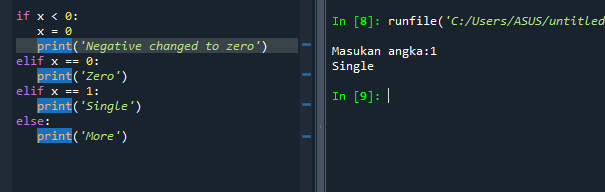
\includegraphics[width=15cm,height=5cm]{image/case7-solved.png}}
    \renewcommand{\figurename}{Gambar}
    \caption{Case-7 Solved}
\end{figure}

% =============================Case 8=============================
\newpage
\section{Case Array String}
\begin{figure}[ht]
    \centerline{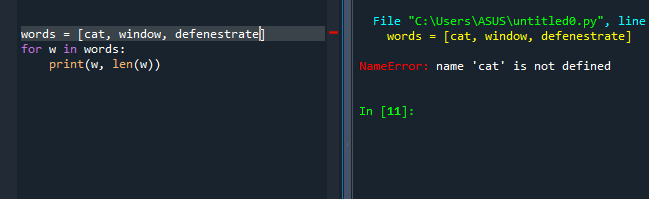
\includegraphics[width=15cm,height=5cm]{image/case8.png}}
    \renewcommand{\figurename}{Gambar}
    \caption{Case-8 Error}
\end{figure}
\paragraph{}\textbf{\textit{Solusi-Case8}} {Cat tidak terdefinisi ketika dijalankan, solusinya yaitu untuk array yang berbentuk string harus menggunakan tanda petik}
\begin{figure}[ht]
    \centerline{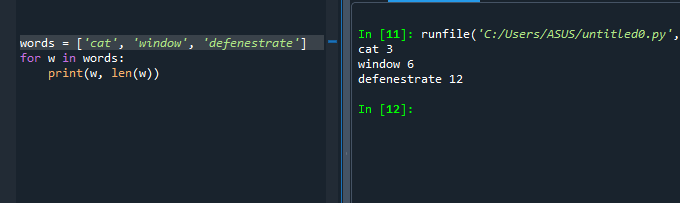
\includegraphics[width=15cm,height=5cm]{image/case8-solved.png}}
    \renewcommand{\figurename}{Gambar}
    \caption{Case-8 Solved}
\end{figure}

% =============================Case 9=============================
\newpage
\section{Case Print Lopping array}
\begin{figure}[ht]
    \centerline{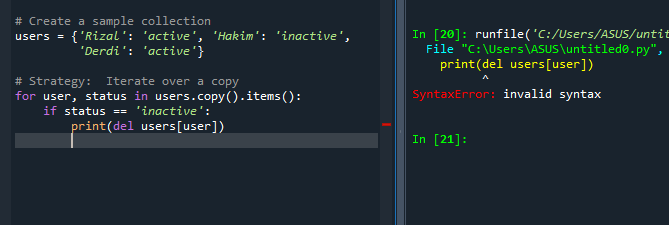
\includegraphics[width=15cm,height=5cm]{image/case9.png}}
    \renewcommand{\figurename}{Gambar}
    \caption{Case-9 Error}
\end{figure}
\paragraph{}\textbf{\textit{Solusi-Case9}} {Kita tidak dapat menggabungkan antara perintah del didalam print, solusianya yaitu dengan memisahkan print yang dimana membawa nilai user. Berikut scriptnya}
\begin{figure}[ht]
    \centerline{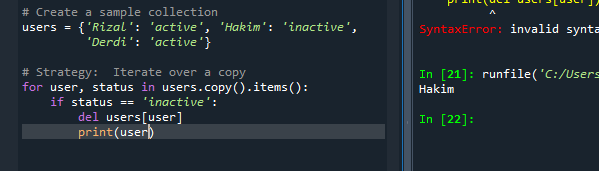
\includegraphics[width=15cm,height=5cm]{image/case9-solved.png}}
    \renewcommand{\figurename}{Gambar}
    \caption{Case-9 Solved}
\end{figure}

% =============================Case 10=============================
\newpage
\section{Case Looping Tipe data}
\begin{figure}[ht]
    \centerline{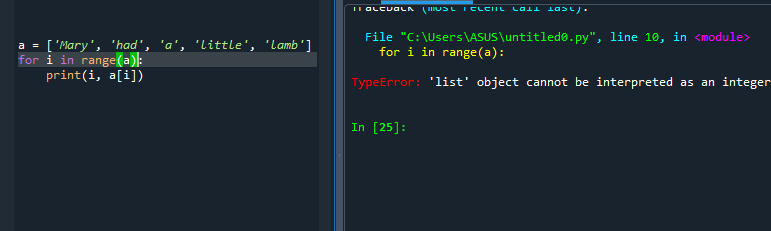
\includegraphics[width=15cm,height=5cm]{image/case10.png}}
    \renewcommand{\figurename}{Gambar}
    \caption{Case-10 Error}
\end{figure}
\paragraph{}\textbf{\textit{Solusi-Case10}} {Kita melihat dalam array terdapat nilai yang berupa string, untuk melakukan perulangan data secara bergantian kita diharuskan untuk menggunakan 'ler' yang memperbolehkan nilai string}
\begin{figure}[ht]
    \centerline{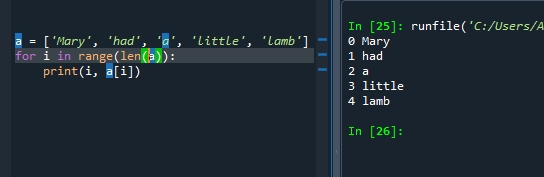
\includegraphics[width=15cm,height=5cm]{image/case10-solved.png}}
    \renewcommand{\figurename}{Gambar}
    \caption{Case-10 Solved}
\end{figure}

% =============================Case 11=============================
\newpage
\section{Case SUM}
\begin{figure}[ht]
    \centerline{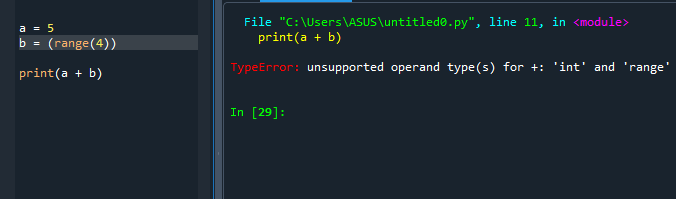
\includegraphics[width=15cm,height=5cm]{image/case11.png}}
    \renewcommand{\figurename}{Gambar}
    \caption{Case-11 Error}
\end{figure}
\paragraph{}\textbf{\textit{Solusi-Case11}} {Untuk menjumlahkan antara angka dengan range angka, maka kita harus menambahkan sum untuk membungkus range}
\begin{figure}[ht]
    \centerline{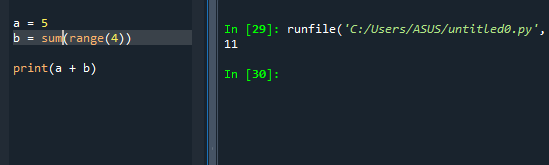
\includegraphics[width=15cm,height=5cm]{image/case11-solved.png}}
    \renewcommand{\figurename}{Gambar}
    \caption{Case-11 Solved}
\end{figure}

% =============================Case 12=============================
\newpage
\section{Case Continue}
\begin{figure}[ht]
    \centerline{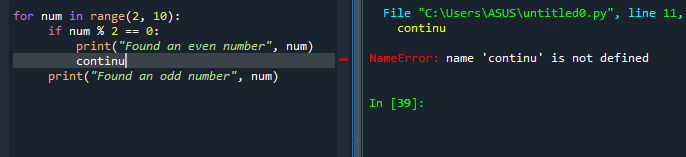
\includegraphics[width=15cm,height=5cm]{image/case12.png}}
    \renewcommand{\figurename}{Gambar}
    \caption{Case-12 Error}
\end{figure}
\paragraph{}\textbf{\textit{Solusi-Case12}} {Untuk melanjutnya eksekusi program kita harus dengan teliti memperhatikan penulisan dari continue}
\begin{figure}[ht]
    \centerline{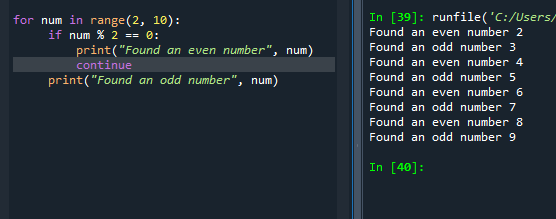
\includegraphics[width=15cm,height=5cm]{image/case12-solved.png}}
    \renewcommand{\figurename}{Gambar}
    \caption{Case-12 Solved}
\end{figure}

% =============================Case 13=============================
\newpage
\section{Case While Conditional}
\begin{figure}[ht]
    \centerline{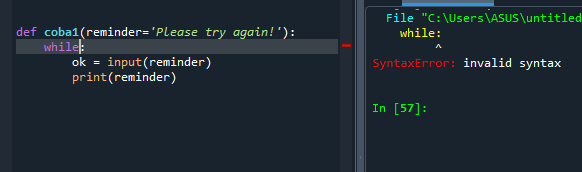
\includegraphics[width=15cm,height=5cm]{image/case13.png}}
    \renewcommand{\figurename}{Gambar}
    \caption{Case-13 Error}
\end{figure}
\paragraph{}\textbf{\textit{Solusi-Case13}} {Menggunakan while condition harus diikutu dengan kondisinya seperti berikut}
\begin{figure}[ht]
    \centerline{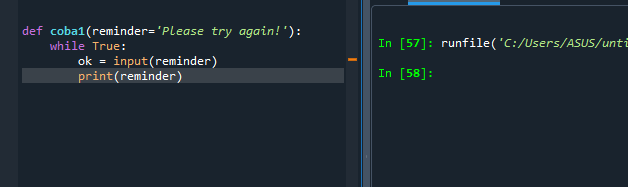
\includegraphics[width=15cm,height=5cm]{image/case13-solved.png}}
    \renewcommand{\figurename}{Gambar}
    \caption{Case-13 Solved}
\end{figure}

% =============================Case 14=============================
\newpage
\section{Case Append}
\begin{figure}[ht]
    \centerline{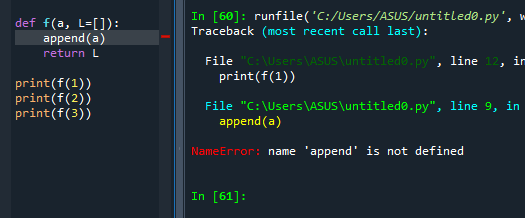
\includegraphics[width=15cm,height=5cm]{image/case14.png}}
    \renewcommand{\figurename}{Gambar}
    \caption{Case-14 Error}
\end{figure}
\paragraph{}\textbf{\textit{Solusi-Case14}} {Syarat menggunakan append yaitu ada variabel terlebih dahulu yang membawa nilai, solusinya mengubah menjadi L.append}
\begin{figure}[ht]
    \centerline{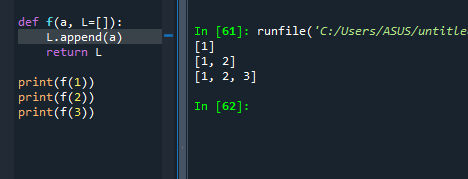
\includegraphics[width=15cm,height=5cm]{image/case14-solved.png}}
    \renewcommand{\figurename}{Gambar}
    \caption{Case-14 Solved}
\end{figure}

% =============================Case 15=============================
\newpage
\section{Case Definition If condition}
\begin{figure}[ht]
    \centerline{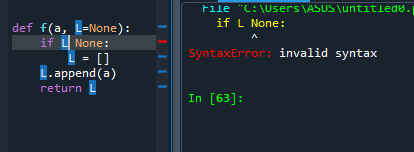
\includegraphics[width=15cm,height=5cm]{image/case15.png}}
    \renewcommand{\figurename}{Gambar}
    \caption{Case-15 Error}
\end{figure}
\paragraph{}\textbf{\textit{Solusi-Case15}} {dalam kondisi if variabel L harus di perjelasan dengan menambahkan penggunaan is .. seperti berikut}
\begin{figure}[ht]
    \centerline{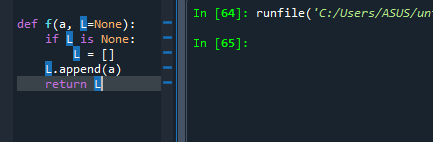
\includegraphics[width=15cm,height=5cm]{image/case15-solved.png}}
    \renewcommand{\figurename}{Gambar}
    \caption{Case-15 Solved}
\end{figure}

% =============================Case 16=============================
\newpage
\section{Case Function}
\begin{figure}[ht]
    \centerline{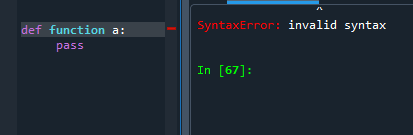
\includegraphics[width=15cm,height=5cm]{image/case16.png}}
    \renewcommand{\figurename}{Gambar}
    \caption{Case-16 Error}
\end{figure}
\paragraph{}\textbf{\textit{Solusi-Case16}} {Dalam penulisan function python nama function harus dibungkus dengan tanda kurung}
\begin{figure}[ht]
    \centerline{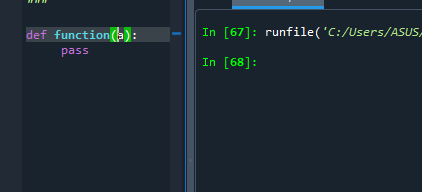
\includegraphics[width=15cm,height=5cm]{image/case16-solved.png}}
    \renewcommand{\figurename}{Gambar}
    \caption{Case-16 Solved}
\end{figure}

% =============================Case 17=============================
\newpage
\section{Case Lambda}
\begin{figure}[ht]
    \centerline{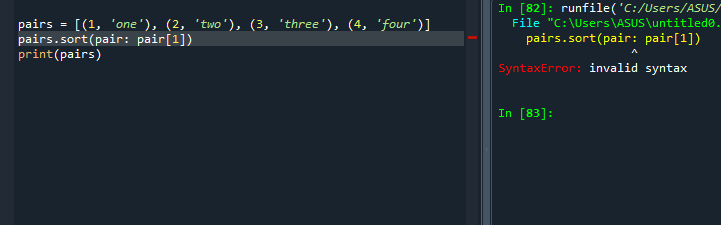
\includegraphics[width=15cm,height=5cm]{image/case17.png}}
    \renewcommand{\figurename}{Gambar}
    \caption{Case-17 Error}
\end{figure}
\paragraph{}\textbf{\textit{Solusi-Case17}} {Untuk memanggil sintak secara berurutan kita harus memanggil atau menggunakan key=lambda}
\begin{figure}[ht]
    \centerline{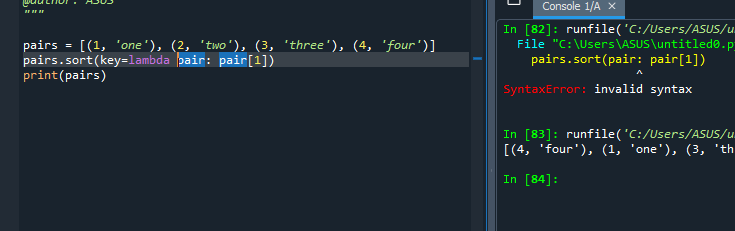
\includegraphics[width=15cm,height=5cm]{image/case17-solved.png}}
    \renewcommand{\figurename}{Gambar}
    \caption{Case-17 Solved}
\end{figure}

% =============================Case 18=============================
\newpage
\section{Case Print Function}
\begin{figure}[ht]
    \centerline{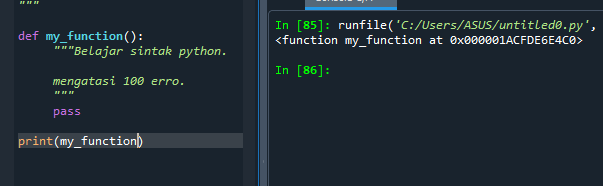
\includegraphics[width=15cm,height=5cm]{image/case18.png}}
    \renewcommand{\figurename}{Gambar}
    \caption{Case-18 Error}
\end{figure}
\paragraph{}\textbf{\textit{Solusi-Case18}} {Untuk menampilkan string multiple baris dengan memanggil function, tentunya bukan hanya print nama function tetapi harus diikutu dengan fungsi doc}
\begin{figure}[ht]
    \centerline{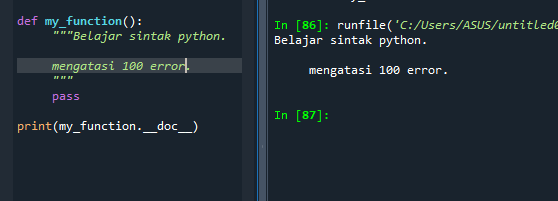
\includegraphics[width=15cm,height=5cm]{image/case18-solved.png}}
    \renewcommand{\figurename}{Gambar}
    \caption{Case-18 Solved}
\end{figure}

% =============================Case 19=============================
\newpage
\section{Case Append}
\begin{figure}[ht]
    \centerline{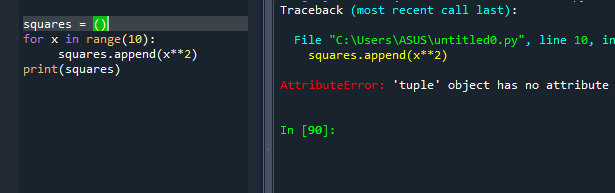
\includegraphics[width=15cm,height=5cm]{image/case19.png}}
    \renewcommand{\figurename}{Gambar}
    \caption{Case-19 Error}
\end{figure}
\paragraph{}\textbf{\textit{Solusi-Case19}} {Dalam penggunaan append kita harus menggunakan kurung siku}
\begin{figure}[ht]
    \centerline{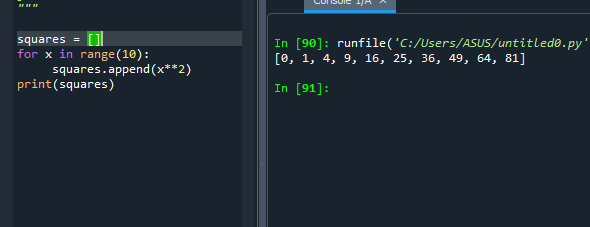
\includegraphics[width=15cm,height=5cm]{image/case19-solved.png}}
    \renewcommand{\figurename}{Gambar}
    \caption{Case-19 Solved}
\end{figure}

% =============================Case 20=============================
\newpage
\section{Case Print}
\begin{figure}[ht]
    \centerline{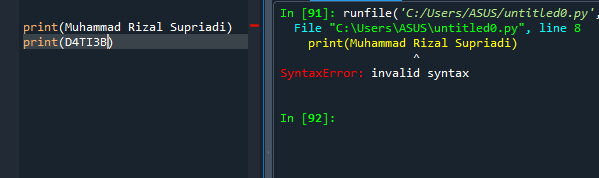
\includegraphics[width=15cm,height=5cm]{image/case20.png}}
    \renewcommand{\figurename}{Gambar}
    \caption{Case-20 Error}
\end{figure}
\paragraph{}\textbf{\textit{Solusi-Case20}} {Print nilai string harus dibungkus dengan tanda petik}
\begin{figure}[ht]
    \centerline{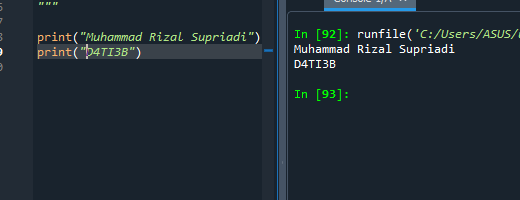
\includegraphics[width=15cm,height=5cm]{image/case20-solved.png}}
    \renewcommand{\figurename}{Gambar}
    \caption{Case-20 Solved}
\end{figure}

% =============================Case 21=============================
\newpage
\section{Case Perkalin}
\begin{figure}[ht]
    \centerline{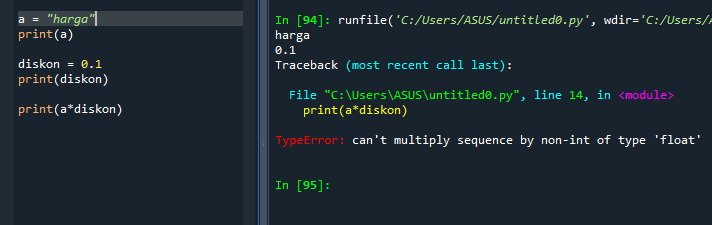
\includegraphics[width=15cm,height=5cm]{image/case21.png}}
    \renewcommand{\figurename}{Gambar}
    \caption{Case-21 Error}
\end{figure}
\paragraph{}\textbf{\textit{Solusi-Case21}} {Error terjadi karena string tidak dapat dikalian dengan integer}
\begin{figure}[ht]
    \centerline{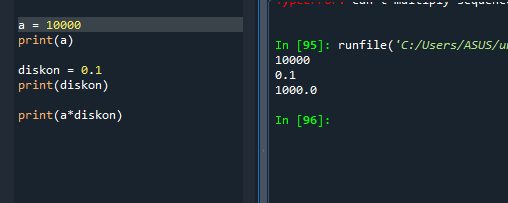
\includegraphics[width=15cm,height=5cm]{image/case21-solved.png}}
    \renewcommand{\figurename}{Gambar}
    \caption{Case-21 Solved}
\end{figure}

% =============================Case 22=============================
\newpage
\section{Case Print}
\begin{figure}[ht]
    \centerline{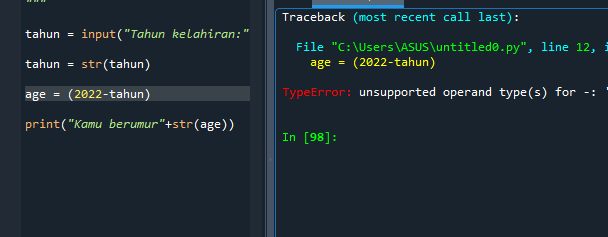
\includegraphics[width=15cm,height=5cm]{image/case22.png}}
    \renewcommand{\figurename}{Gambar}
    \caption{Case-22 Error}
\end{figure}
\paragraph{}\textbf{\textit{Solusi-Case22}} {Untuk melakukan perulangan str(tahun) harus diganti menjadi int(tahun)}
\begin{figure}[ht]
    \centerline{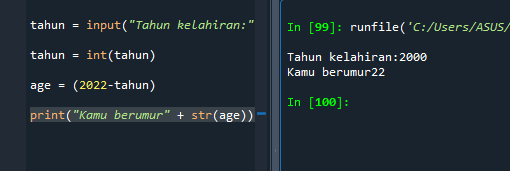
\includegraphics[width=15cm,height=5cm]{image/case22-solved.png}}
    \renewcommand{\figurename}{Gambar}
    \caption{Case-22 Solved}
\end{figure}

% =============================Case 23=============================
\newpage
\section{Case Kurung Kurawal}
\begin{figure}[ht]
    \centerline{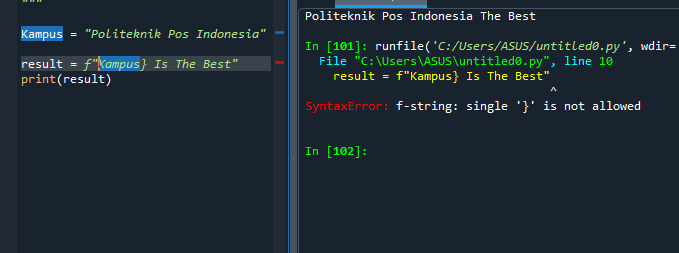
\includegraphics[width=15cm,height=5cm]{image/case23.png}}
    \renewcommand{\figurename}{Gambar}
    \caption{Case-23 Error}
\end{figure}
\paragraph{}\textbf{\textit{Solusi-Case23}} {Error terjadi karena saya tidak membuka dengan kurung kurawal untuk Kampus}
\begin{figure}[ht]
    \centerline{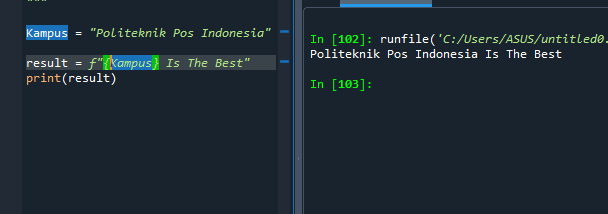
\includegraphics[width=15cm,height=5cm]{image/case23-solved.png}}
    \renewcommand{\figurename}{Gambar}
    \caption{Case-23 Solved}
\end{figure}

% =============================Case 24=============================
\newpage
\section{Case Math}
\begin{figure}[ht]
    \centerline{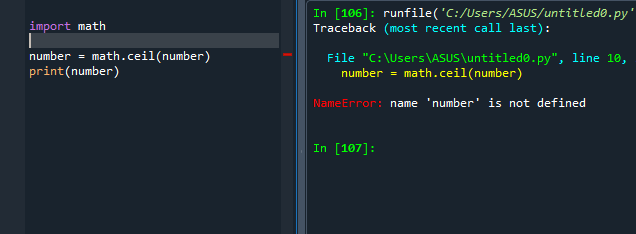
\includegraphics[width=15cm,height=5cm]{image/case24.png}}
    \renewcommand{\figurename}{Gambar}
    \caption{Case-24 Error}
\end{figure}
\paragraph{}\textbf{\textit{Solusi-Case24}} {Number belum didefinisikan jadi belum terdapat nilai}
\begin{figure}[ht]
    \centerline{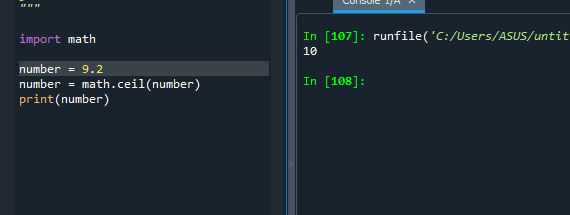
\includegraphics[width=15cm,height=5cm]{image/case24-solved.png}}
    \renewcommand{\figurename}{Gambar}
    \caption{Case-24 Solved}
\end{figure}

% =============================Case 25=============================
\newpage
\section{Case IF}
\begin{figure}[ht]
    \centerline{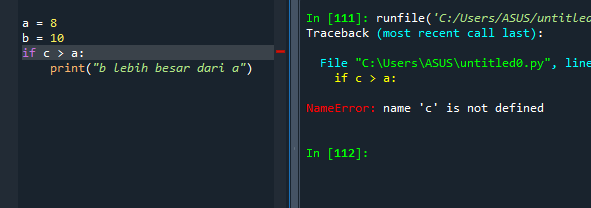
\includegraphics[width=15cm,height=5cm]{image/case25.png}}
    \renewcommand{\figurename}{Gambar}
    \caption{Case-25 Error}
\end{figure}
\paragraph{}\textbf{\textit{Solusi-Case25}} {variabel c tidak terdefinisi dan harus di singkronkan}
\begin{figure}[ht]
    \centerline{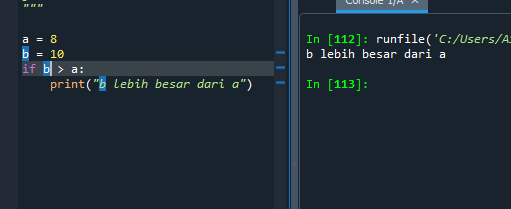
\includegraphics[width=15cm,height=5cm]{image/case25-solved.png}}
    \renewcommand{\figurename}{Gambar}
    \caption{Case-25 Solved}
\end{figure}

% =============================Case 26=============================
\newpage
\section{Case Print}
\begin{figure}[ht]
    \centerline{\includegraphics[width=15cm,height=5cm]{image/case6.png}}
    \renewcommand{\figurename}{Gambar}
    \caption{Case-6 Error}
\end{figure}
\paragraph{}\textbf{\textit{Solusi-Case6}} {Ketika kita print beberapa baris secara langsung, maka yang harus dilakukan adalah dengan menggunakan petik 2 .. 3 kali... berikut contoh yang benar}
\begin{figure}[ht]
    \centerline{\includegraphics[width=15cm,height=5cm]{image/case6-solved.png}}
    \renewcommand{\figurename}{Gambar}
    \caption{Case-6 Solved}
\end{figure}

% =============================Case 27=============================
\newpage
\section{Case Print}
\begin{figure}[ht]
    \centerline{\includegraphics[width=15cm,height=5cm]{image/case6.png}}
    \renewcommand{\figurename}{Gambar}
    \caption{Case-6 Error}
\end{figure}
\paragraph{}\textbf{\textit{Solusi-Case6}} {Ketika kita print beberapa baris secara langsung, maka yang harus dilakukan adalah dengan menggunakan petik 2 .. 3 kali... berikut contoh yang benar}
\begin{figure}[ht]
    \centerline{\includegraphics[width=15cm,height=5cm]{image/case6-solved.png}}
    \renewcommand{\figurename}{Gambar}
    \caption{Case-6 Solved}
\end{figure}

% =============================Case 28=============================
\newpage
\section{Case Print}
\begin{figure}[ht]
    \centerline{\includegraphics[width=15cm,height=5cm]{image/case6.png}}
    \renewcommand{\figurename}{Gambar}
    \caption{Case-6 Error}
\end{figure}
\paragraph{}\textbf{\textit{Solusi-Case6}} {Ketika kita print beberapa baris secara langsung, maka yang harus dilakukan adalah dengan menggunakan petik 2 .. 3 kali... berikut contoh yang benar}
\begin{figure}[ht]
    \centerline{\includegraphics[width=15cm,height=5cm]{image/case6-solved.png}}
    \renewcommand{\figurename}{Gambar}
    \caption{Case-6 Solved}
\end{figure}

% =============================Case 29=============================
\newpage
\section{Case Print}
\begin{figure}[ht]
    \centerline{\includegraphics[width=15cm,height=5cm]{image/case6.png}}
    \renewcommand{\figurename}{Gambar}
    \caption{Case-6 Error}
\end{figure}
\paragraph{}\textbf{\textit{Solusi-Case6}} {Ketika kita print beberapa baris secara langsung, maka yang harus dilakukan adalah dengan menggunakan petik 2 .. 3 kali... berikut contoh yang benar}
\begin{figure}[ht]
    \centerline{\includegraphics[width=15cm,height=5cm]{image/case6-solved.png}}
    \renewcommand{\figurename}{Gambar}
    \caption{Case-6 Solved}
\end{figure}

% =============================Case 30=============================
\newpage
\section{Case Print}
\begin{figure}[ht]
    \centerline{\includegraphics[width=15cm,height=5cm]{image/case6.png}}
    \renewcommand{\figurename}{Gambar}
    \caption{Case-6 Error}
\end{figure}
\paragraph{}\textbf{\textit{Solusi-Case6}} {Ketika kita print beberapa baris secara langsung, maka yang harus dilakukan adalah dengan menggunakan petik 2 .. 3 kali... berikut contoh yang benar}
\begin{figure}[ht]
    \centerline{\includegraphics[width=15cm,height=5cm]{image/case6-solved.png}}
    \renewcommand{\figurename}{Gambar}
    \caption{Case-6 Solved}
\end{figure}

% =============================Case 31=============================
\newpage
\section{Case Print}
\begin{figure}[ht]
    \centerline{\includegraphics[width=15cm,height=5cm]{image/case6.png}}
    \renewcommand{\figurename}{Gambar}
    \caption{Case-6 Error}
\end{figure}
\paragraph{}\textbf{\textit{Solusi-Case6}} {Ketika kita print beberapa baris secara langsung, maka yang harus dilakukan adalah dengan menggunakan petik 2 .. 3 kali... berikut contoh yang benar}
\begin{figure}[ht]
    \centerline{\includegraphics[width=15cm,height=5cm]{image/case6-solved.png}}
    \renewcommand{\figurename}{Gambar}
    \caption{Case-6 Solved}
\end{figure}

% =============================Case 32=============================
\newpage
\section{Case Print}
\begin{figure}[ht]
    \centerline{\includegraphics[width=15cm,height=5cm]{image/case6.png}}
    \renewcommand{\figurename}{Gambar}
    \caption{Case-6 Error}
\end{figure}
\paragraph{}\textbf{\textit{Solusi-Case6}} {Ketika kita print beberapa baris secara langsung, maka yang harus dilakukan adalah dengan menggunakan petik 2 .. 3 kali... berikut contoh yang benar}
\begin{figure}[ht]
    \centerline{\includegraphics[width=15cm,height=5cm]{image/case6-solved.png}}
    \renewcommand{\figurename}{Gambar}
    \caption{Case-6 Solved}
\end{figure}

% =============================Case 33=============================
\newpage
\section{Case Print}
\begin{figure}[ht]
    \centerline{\includegraphics[width=15cm,height=5cm]{image/case6.png}}
    \renewcommand{\figurename}{Gambar}
    \caption{Case-6 Error}
\end{figure}
\paragraph{}\textbf{\textit{Solusi-Case6}} {Ketika kita print beberapa baris secara langsung, maka yang harus dilakukan adalah dengan menggunakan petik 2 .. 3 kali... berikut contoh yang benar}
\begin{figure}[ht]
    \centerline{\includegraphics[width=15cm,height=5cm]{image/case6-solved.png}}
    \renewcommand{\figurename}{Gambar}
    \caption{Case-6 Solved}
\end{figure}

% =============================Case 34=============================
\newpage
\section{Case Print}
\begin{figure}[ht]
    \centerline{\includegraphics[width=15cm,height=5cm]{image/case6.png}}
    \renewcommand{\figurename}{Gambar}
    \caption{Case-6 Error}
\end{figure}
\paragraph{}\textbf{\textit{Solusi-Case6}} {Ketika kita print beberapa baris secara langsung, maka yang harus dilakukan adalah dengan menggunakan petik 2 .. 3 kali... berikut contoh yang benar}
\begin{figure}[ht]
    \centerline{\includegraphics[width=15cm,height=5cm]{image/case6-solved.png}}
    \renewcommand{\figurename}{Gambar}
    \caption{Case-6 Solved}
\end{figure}

% =============================Case 35=============================
\newpage
\section{Case Print}
\begin{figure}[ht]
    \centerline{\includegraphics[width=15cm,height=5cm]{image/case6.png}}
    \renewcommand{\figurename}{Gambar}
    \caption{Case-6 Error}
\end{figure}
\paragraph{}\textbf{\textit{Solusi-Case6}} {Ketika kita print beberapa baris secara langsung, maka yang harus dilakukan adalah dengan menggunakan petik 2 .. 3 kali... berikut contoh yang benar}
\begin{figure}[ht]
    \centerline{\includegraphics[width=15cm,height=5cm]{image/case6-solved.png}}
    \renewcommand{\figurename}{Gambar}
    \caption{Case-6 Solved}
\end{figure}

% =============================Case 36=============================
\newpage
\section{Case Print}
\begin{figure}[ht]
    \centerline{\includegraphics[width=15cm,height=5cm]{image/case6.png}}
    \renewcommand{\figurename}{Gambar}
    \caption{Case-6 Error}
\end{figure}
\paragraph{}\textbf{\textit{Solusi-Case6}} {Ketika kita print beberapa baris secara langsung, maka yang harus dilakukan adalah dengan menggunakan petik 2 .. 3 kali... berikut contoh yang benar}
\begin{figure}[ht]
    \centerline{\includegraphics[width=15cm,height=5cm]{image/case6-solved.png}}
    \renewcommand{\figurename}{Gambar}
    \caption{Case-6 Solved}
\end{figure}

% =============================Case 37=============================
\newpage
\section{Case Print}
\begin{figure}[ht]
    \centerline{\includegraphics[width=15cm,height=5cm]{image/case6.png}}
    \renewcommand{\figurename}{Gambar}
    \caption{Case-6 Error}
\end{figure}
\paragraph{}\textbf{\textit{Solusi-Case6}} {Ketika kita print beberapa baris secara langsung, maka yang harus dilakukan adalah dengan menggunakan petik 2 .. 3 kali... berikut contoh yang benar}
\begin{figure}[ht]
    \centerline{\includegraphics[width=15cm,height=5cm]{image/case6-solved.png}}
    \renewcommand{\figurename}{Gambar}
    \caption{Case-6 Solved}
\end{figure}

% =============================Case 38=============================
\newpage
\section{Case Print}
\begin{figure}[ht]
    \centerline{\includegraphics[width=15cm,height=5cm]{image/case6.png}}
    \renewcommand{\figurename}{Gambar}
    \caption{Case-6 Error}
\end{figure}
\paragraph{}\textbf{\textit{Solusi-Case6}} {Ketika kita print beberapa baris secara langsung, maka yang harus dilakukan adalah dengan menggunakan petik 2 .. 3 kali... berikut contoh yang benar}
\begin{figure}[ht]
    \centerline{\includegraphics[width=15cm,height=5cm]{image/case6-solved.png}}
    \renewcommand{\figurename}{Gambar}
    \caption{Case-6 Solved}
\end{figure}

% =============================Case 39=============================
\newpage
\section{Case Print}
\begin{figure}[ht]
    \centerline{\includegraphics[width=15cm,height=5cm]{image/case6.png}}
    \renewcommand{\figurename}{Gambar}
    \caption{Case-6 Error}
\end{figure}
\paragraph{}\textbf{\textit{Solusi-Case6}} {Ketika kita print beberapa baris secara langsung, maka yang harus dilakukan adalah dengan menggunakan petik 2 .. 3 kali... berikut contoh yang benar}
\begin{figure}[ht]
    \centerline{\includegraphics[width=15cm,height=5cm]{image/case6-solved.png}}
    \renewcommand{\figurename}{Gambar}
    \caption{Case-6 Solved}
\end{figure}

% =============================Case 40=============================
\newpage
\section{Case Print}
\begin{figure}[ht]
    \centerline{\includegraphics[width=15cm,height=5cm]{image/case6.png}}
    \renewcommand{\figurename}{Gambar}
    \caption{Case-6 Error}
\end{figure}
\paragraph{}\textbf{\textit{Solusi-Case6}} {Ketika kita print beberapa baris secara langsung, maka yang harus dilakukan adalah dengan menggunakan petik 2 .. 3 kali... berikut contoh yang benar}
\begin{figure}[ht]
    \centerline{\includegraphics[width=15cm,height=5cm]{image/case6-solved.png}}
    \renewcommand{\figurename}{Gambar}
    \caption{Case-6 Solved}
\end{figure}

% =============================Case 41=============================
\newpage
\section{Case Print}
\begin{figure}[ht]
    \centerline{\includegraphics[width=15cm,height=5cm]{image/case6.png}}
    \renewcommand{\figurename}{Gambar}
    \caption{Case-6 Error}
\end{figure}
\paragraph{}\textbf{\textit{Solusi-Case6}} {Ketika kita print beberapa baris secara langsung, maka yang harus dilakukan adalah dengan menggunakan petik 2 .. 3 kali... berikut contoh yang benar}
\begin{figure}[ht]
    \centerline{\includegraphics[width=15cm,height=5cm]{image/case6-solved.png}}
    \renewcommand{\figurename}{Gambar}
    \caption{Case-6 Solved}
\end{figure}

% =============================Case 42=============================
\newpage
\section{Case Print}
\begin{figure}[ht]
    \centerline{\includegraphics[width=15cm,height=5cm]{image/case6.png}}
    \renewcommand{\figurename}{Gambar}
    \caption{Case-6 Error}
\end{figure}
\paragraph{}\textbf{\textit{Solusi-Case6}} {Ketika kita print beberapa baris secara langsung, maka yang harus dilakukan adalah dengan menggunakan petik 2 .. 3 kali... berikut contoh yang benar}
\begin{figure}[ht]
    \centerline{\includegraphics[width=15cm,height=5cm]{image/case6-solved.png}}
    \renewcommand{\figurename}{Gambar}
    \caption{Case-6 Solved}
\end{figure}

% =============================Case 43=============================
\newpage
\section{Case Print}
\begin{figure}[ht]
    \centerline{\includegraphics[width=15cm,height=5cm]{image/case6.png}}
    \renewcommand{\figurename}{Gambar}
    \caption{Case-6 Error}
\end{figure}
\paragraph{}\textbf{\textit{Solusi-Case6}} {Ketika kita print beberapa baris secara langsung, maka yang harus dilakukan adalah dengan menggunakan petik 2 .. 3 kali... berikut contoh yang benar}
\begin{figure}[ht]
    \centerline{\includegraphics[width=15cm,height=5cm]{image/case6-solved.png}}
    \renewcommand{\figurename}{Gambar}
    \caption{Case-6 Solved}
\end{figure}

% =============================Case 44=============================
\newpage
\section{Case Print}
\begin{figure}[ht]
    \centerline{\includegraphics[width=15cm,height=5cm]{image/case6.png}}
    \renewcommand{\figurename}{Gambar}
    \caption{Case-6 Error}
\end{figure}
\paragraph{}\textbf{\textit{Solusi-Case6}} {Ketika kita print beberapa baris secara langsung, maka yang harus dilakukan adalah dengan menggunakan petik 2 .. 3 kali... berikut contoh yang benar}
\begin{figure}[ht]
    \centerline{\includegraphics[width=15cm,height=5cm]{image/case6-solved.png}}
    \renewcommand{\figurename}{Gambar}
    \caption{Case-6 Solved}
\end{figure}

% =============================Case 45=============================
\newpage
\section{Case Print}
\begin{figure}[ht]
    \centerline{\includegraphics[width=15cm,height=5cm]{image/case6.png}}
    \renewcommand{\figurename}{Gambar}
    \caption{Case-6 Error}
\end{figure}
\paragraph{}\textbf{\textit{Solusi-Case6}} {Ketika kita print beberapa baris secara langsung, maka yang harus dilakukan adalah dengan menggunakan petik 2 .. 3 kali... berikut contoh yang benar}
\begin{figure}[ht]
    \centerline{\includegraphics[width=15cm,height=5cm]{image/case6-solved.png}}
    \renewcommand{\figurename}{Gambar}
    \caption{Case-6 Solved}
\end{figure}

% =============================Case 46=============================
\newpage
\section{Case Print}
\begin{figure}[ht]
    \centerline{\includegraphics[width=15cm,height=5cm]{image/case6.png}}
    \renewcommand{\figurename}{Gambar}
    \caption{Case-6 Error}
\end{figure}
\paragraph{}\textbf{\textit{Solusi-Case6}} {Ketika kita print beberapa baris secara langsung, maka yang harus dilakukan adalah dengan menggunakan petik 2 .. 3 kali... berikut contoh yang benar}
\begin{figure}[ht]
    \centerline{\includegraphics[width=15cm,height=5cm]{image/case6-solved.png}}
    \renewcommand{\figurename}{Gambar}
    \caption{Case-6 Solved}
\end{figure}

% =============================Case 47=============================
\newpage
\section{Case Print}
\begin{figure}[ht]
    \centerline{\includegraphics[width=15cm,height=5cm]{image/case6.png}}
    \renewcommand{\figurename}{Gambar}
    \caption{Case-6 Error}
\end{figure}
\paragraph{}\textbf{\textit{Solusi-Case6}} {Ketika kita print beberapa baris secara langsung, maka yang harus dilakukan adalah dengan menggunakan petik 2 .. 3 kali... berikut contoh yang benar}
\begin{figure}[ht]
    \centerline{\includegraphics[width=15cm,height=5cm]{image/case6-solved.png}}
    \renewcommand{\figurename}{Gambar}
    \caption{Case-6 Solved}
\end{figure}

% =============================Case 48=============================
\newpage
\section{Case Print}
\begin{figure}[ht]
    \centerline{\includegraphics[width=15cm,height=5cm]{image/case6.png}}
    \renewcommand{\figurename}{Gambar}
    \caption{Case-6 Error}
\end{figure}
\paragraph{}\textbf{\textit{Solusi-Case6}} {Ketika kita print beberapa baris secara langsung, maka yang harus dilakukan adalah dengan menggunakan petik 2 .. 3 kali... berikut contoh yang benar}
\begin{figure}[ht]
    \centerline{\includegraphics[width=15cm,height=5cm]{image/case6-solved.png}}
    \renewcommand{\figurename}{Gambar}
    \caption{Case-6 Solved}
\end{figure}

% =============================Case 49=============================
\newpage
\section{Case Print}
\begin{figure}[ht]
    \centerline{\includegraphics[width=15cm,height=5cm]{image/case6.png}}
    \renewcommand{\figurename}{Gambar}
    \caption{Case-6 Error}
\end{figure}
\paragraph{}\textbf{\textit{Solusi-Case6}} {Ketika kita print beberapa baris secara langsung, maka yang harus dilakukan adalah dengan menggunakan petik 2 .. 3 kali... berikut contoh yang benar}
\begin{figure}[ht]
    \centerline{\includegraphics[width=15cm,height=5cm]{image/case6-solved.png}}
    \renewcommand{\figurename}{Gambar}
    \caption{Case-6 Solved}
\end{figure}

% =============================Case 50=============================
\newpage
\section{Case Print}
\begin{figure}[ht]
    \centerline{\includegraphics[width=15cm,height=5cm]{image/case6.png}}
    \renewcommand{\figurename}{Gambar}
    \caption{Case-6 Error}
\end{figure}
\paragraph{}\textbf{\textit{Solusi-Case6}} {Ketika kita print beberapa baris secara langsung, maka yang harus dilakukan adalah dengan menggunakan petik 2 .. 3 kali... berikut contoh yang benar}
\begin{figure}[ht]
    \centerline{\includegraphics[width=15cm,height=5cm]{image/case6-solved.png}}
    \renewcommand{\figurename}{Gambar}
    \caption{Case-6 Solved}
\end{figure}

% =============================Case 51=============================
\newpage
\section{Case Print}
\begin{figure}[ht]
    \centerline{\includegraphics[width=15cm,height=5cm]{image/case6.png}}
    \renewcommand{\figurename}{Gambar}
    \caption{Case-6 Error}
\end{figure}
\paragraph{}\textbf{\textit{Solusi-Case6}} {Ketika kita print beberapa baris secara langsung, maka yang harus dilakukan adalah dengan menggunakan petik 2 .. 3 kali... berikut contoh yang benar}
\begin{figure}[ht]
    \centerline{\includegraphics[width=15cm,height=5cm]{image/case6-solved.png}}
    \renewcommand{\figurename}{Gambar}
    \caption{Case-6 Solved}
\end{figure}

% =============================Case 52=============================
\newpage
\section{Case Print}
\begin{figure}[ht]
    \centerline{\includegraphics[width=15cm,height=5cm]{image/case6.png}}
    \renewcommand{\figurename}{Gambar}
    \caption{Case-6 Error}
\end{figure}
\paragraph{}\textbf{\textit{Solusi-Case6}} {Ketika kita print beberapa baris secara langsung, maka yang harus dilakukan adalah dengan menggunakan petik 2 .. 3 kali... berikut contoh yang benar}
\begin{figure}[ht]
    \centerline{\includegraphics[width=15cm,height=5cm]{image/case6-solved.png}}
    \renewcommand{\figurename}{Gambar}
    \caption{Case-6 Solved}
\end{figure}

% =============================Case 53=============================
\newpage
\section{Case Print}
\begin{figure}[ht]
    \centerline{\includegraphics[width=15cm,height=5cm]{image/case6.png}}
    \renewcommand{\figurename}{Gambar}
    \caption{Case-6 Error}
\end{figure}
\paragraph{}\textbf{\textit{Solusi-Case6}} {Ketika kita print beberapa baris secara langsung, maka yang harus dilakukan adalah dengan menggunakan petik 2 .. 3 kali... berikut contoh yang benar}
\begin{figure}[ht]
    \centerline{\includegraphics[width=15cm,height=5cm]{image/case6-solved.png}}
    \renewcommand{\figurename}{Gambar}
    \caption{Case-6 Solved}
\end{figure}

% =============================Case 54=============================
\newpage
\section{Case Print}
\begin{figure}[ht]
    \centerline{\includegraphics[width=15cm,height=5cm]{image/case6.png}}
    \renewcommand{\figurename}{Gambar}
    \caption{Case-6 Error}
\end{figure}
\paragraph{}\textbf{\textit{Solusi-Case6}} {Ketika kita print beberapa baris secara langsung, maka yang harus dilakukan adalah dengan menggunakan petik 2 .. 3 kali... berikut contoh yang benar}
\begin{figure}[ht]
    \centerline{\includegraphics[width=15cm,height=5cm]{image/case6-solved.png}}
    \renewcommand{\figurename}{Gambar}
    \caption{Case-6 Solved}
\end{figure}

% =============================Case 55=============================
\newpage
\section{Case Print}
\begin{figure}[ht]
    \centerline{\includegraphics[width=15cm,height=5cm]{image/case6.png}}
    \renewcommand{\figurename}{Gambar}
    \caption{Case-6 Error}
\end{figure}
\paragraph{}\textbf{\textit{Solusi-Case6}} {Ketika kita print beberapa baris secara langsung, maka yang harus dilakukan adalah dengan menggunakan petik 2 .. 3 kali... berikut contoh yang benar}
\begin{figure}[ht]
    \centerline{\includegraphics[width=15cm,height=5cm]{image/case6-solved.png}}
    \renewcommand{\figurename}{Gambar}
    \caption{Case-6 Solved}
\end{figure}

% =============================Case 56=============================
\newpage
\section{Case Print}
\begin{figure}[ht]
    \centerline{\includegraphics[width=15cm,height=5cm]{image/case6.png}}
    \renewcommand{\figurename}{Gambar}
    \caption{Case-6 Error}
\end{figure}
\paragraph{}\textbf{\textit{Solusi-Case6}} {Ketika kita print beberapa baris secara langsung, maka yang harus dilakukan adalah dengan menggunakan petik 2 .. 3 kali... berikut contoh yang benar}
\begin{figure}[ht]
    \centerline{\includegraphics[width=15cm,height=5cm]{image/case6-solved.png}}
    \renewcommand{\figurename}{Gambar}
    \caption{Case-6 Solved}
\end{figure}

% =============================Case 57=============================
\newpage
\section{Case Print}
\begin{figure}[ht]
    \centerline{\includegraphics[width=15cm,height=5cm]{image/case6.png}}
    \renewcommand{\figurename}{Gambar}
    \caption{Case-6 Error}
\end{figure}
\paragraph{}\textbf{\textit{Solusi-Case6}} {Ketika kita print beberapa baris secara langsung, maka yang harus dilakukan adalah dengan menggunakan petik 2 .. 3 kali... berikut contoh yang benar}
\begin{figure}[ht]
    \centerline{\includegraphics[width=15cm,height=5cm]{image/case6-solved.png}}
    \renewcommand{\figurename}{Gambar}
    \caption{Case-6 Solved}
\end{figure}

% =============================Case 58=============================
\newpage
\section{Case Print}
\begin{figure}[ht]
    \centerline{\includegraphics[width=15cm,height=5cm]{image/case6.png}}
    \renewcommand{\figurename}{Gambar}
    \caption{Case-6 Error}
\end{figure}
\paragraph{}\textbf{\textit{Solusi-Case6}} {Ketika kita print beberapa baris secara langsung, maka yang harus dilakukan adalah dengan menggunakan petik 2 .. 3 kali... berikut contoh yang benar}
\begin{figure}[ht]
    \centerline{\includegraphics[width=15cm,height=5cm]{image/case6-solved.png}}
    \renewcommand{\figurename}{Gambar}
    \caption{Case-6 Solved}
\end{figure}

% =============================Case 59=============================
\newpage
\section{Case Print}
\begin{figure}[ht]
    \centerline{\includegraphics[width=15cm,height=5cm]{image/case6.png}}
    \renewcommand{\figurename}{Gambar}
    \caption{Case-6 Error}
\end{figure}
\paragraph{}\textbf{\textit{Solusi-Case6}} {Ketika kita print beberapa baris secara langsung, maka yang harus dilakukan adalah dengan menggunakan petik 2 .. 3 kali... berikut contoh yang benar}
\begin{figure}[ht]
    \centerline{\includegraphics[width=15cm,height=5cm]{image/case6-solved.png}}
    \renewcommand{\figurename}{Gambar}
    \caption{Case-6 Solved}
\end{figure}

% =============================Case 60=============================
\newpage
\section{Case Print}
\begin{figure}[ht]
    \centerline{\includegraphics[width=15cm,height=5cm]{image/case6.png}}
    \renewcommand{\figurename}{Gambar}
    \caption{Case-6 Error}
\end{figure}
\paragraph{}\textbf{\textit{Solusi-Case6}} {Ketika kita print beberapa baris secara langsung, maka yang harus dilakukan adalah dengan menggunakan petik 2 .. 3 kali... berikut contoh yang benar}
\begin{figure}[ht]
    \centerline{\includegraphics[width=15cm,height=5cm]{image/case6-solved.png}}
    \renewcommand{\figurename}{Gambar}
    \caption{Case-6 Solved}
\end{figure}

% =============================Case 61=============================
\newpage
\section{Case Print}
\begin{figure}[ht]
    \centerline{\includegraphics[width=15cm,height=5cm]{image/case6.png}}
    \renewcommand{\figurename}{Gambar}
    \caption{Case-6 Error}
\end{figure}
\paragraph{}\textbf{\textit{Solusi-Case6}} {Ketika kita print beberapa baris secara langsung, maka yang harus dilakukan adalah dengan menggunakan petik 2 .. 3 kali... berikut contoh yang benar}
\begin{figure}[ht]
    \centerline{\includegraphics[width=15cm,height=5cm]{image/case6-solved.png}}
    \renewcommand{\figurename}{Gambar}
    \caption{Case-6 Solved}
\end{figure}

% =============================Case 62=============================
\newpage
\section{Case Print}
\begin{figure}[ht]
    \centerline{\includegraphics[width=15cm,height=5cm]{image/case6.png}}
    \renewcommand{\figurename}{Gambar}
    \caption{Case-6 Error}
\end{figure}
\paragraph{}\textbf{\textit{Solusi-Case6}} {Ketika kita print beberapa baris secara langsung, maka yang harus dilakukan adalah dengan menggunakan petik 2 .. 3 kali... berikut contoh yang benar}
\begin{figure}[ht]
    \centerline{\includegraphics[width=15cm,height=5cm]{image/case6-solved.png}}
    \renewcommand{\figurename}{Gambar}
    \caption{Case-6 Solved}
\end{figure}

% =============================Case 63=============================
\newpage
\section{Case Print}
\begin{figure}[ht]
    \centerline{\includegraphics[width=15cm,height=5cm]{image/case6.png}}
    \renewcommand{\figurename}{Gambar}
    \caption{Case-6 Error}
\end{figure}
\paragraph{}\textbf{\textit{Solusi-Case6}} {Ketika kita print beberapa baris secara langsung, maka yang harus dilakukan adalah dengan menggunakan petik 2 .. 3 kali... berikut contoh yang benar}
\begin{figure}[ht]
    \centerline{\includegraphics[width=15cm,height=5cm]{image/case6-solved.png}}
    \renewcommand{\figurename}{Gambar}
    \caption{Case-6 Solved}
\end{figure}

% =============================Case 64=============================
\newpage
\section{Case Print}
\begin{figure}[ht]
    \centerline{\includegraphics[width=15cm,height=5cm]{image/case6.png}}
    \renewcommand{\figurename}{Gambar}
    \caption{Case-6 Error}
\end{figure}
\paragraph{}\textbf{\textit{Solusi-Case6}} {Ketika kita print beberapa baris secara langsung, maka yang harus dilakukan adalah dengan menggunakan petik 2 .. 3 kali... berikut contoh yang benar}
\begin{figure}[ht]
    \centerline{\includegraphics[width=15cm,height=5cm]{image/case6-solved.png}}
    \renewcommand{\figurename}{Gambar}
    \caption{Case-6 Solved}
\end{figure}

% =============================Case 65=============================
\newpage
\section{Case Print}
\begin{figure}[ht]
    \centerline{\includegraphics[width=15cm,height=5cm]{image/case6.png}}
    \renewcommand{\figurename}{Gambar}
    \caption{Case-6 Error}
\end{figure}
\paragraph{}\textbf{\textit{Solusi-Case6}} {Ketika kita print beberapa baris secara langsung, maka yang harus dilakukan adalah dengan menggunakan petik 2 .. 3 kali... berikut contoh yang benar}
\begin{figure}[ht]
    \centerline{\includegraphics[width=15cm,height=5cm]{image/case6-solved.png}}
    \renewcommand{\figurename}{Gambar}
    \caption{Case-6 Solved}
\end{figure}

% =============================Case 66=============================
\newpage
\section{Case Print}
\begin{figure}[ht]
    \centerline{\includegraphics[width=15cm,height=5cm]{image/case6.png}}
    \renewcommand{\figurename}{Gambar}
    \caption{Case-6 Error}
\end{figure}
\paragraph{}\textbf{\textit{Solusi-Case6}} {Ketika kita print beberapa baris secara langsung, maka yang harus dilakukan adalah dengan menggunakan petik 2 .. 3 kali... berikut contoh yang benar}
\begin{figure}[ht]
    \centerline{\includegraphics[width=15cm,height=5cm]{image/case6-solved.png}}
    \renewcommand{\figurename}{Gambar}
    \caption{Case-6 Solved}
\end{figure}

% =============================Case 67=============================
\newpage
\section{Case Print}
\begin{figure}[ht]
    \centerline{\includegraphics[width=15cm,height=5cm]{image/case6.png}}
    \renewcommand{\figurename}{Gambar}
    \caption{Case-6 Error}
\end{figure}
\paragraph{}\textbf{\textit{Solusi-Case6}} {Ketika kita print beberapa baris secara langsung, maka yang harus dilakukan adalah dengan menggunakan petik 2 .. 3 kali... berikut contoh yang benar}
\begin{figure}[ht]
    \centerline{\includegraphics[width=15cm,height=5cm]{image/case6-solved.png}}
    \renewcommand{\figurename}{Gambar}
    \caption{Case-6 Solved}
\end{figure}

% =============================Case 68=============================
\newpage
\section{Case Print}
\begin{figure}[ht]
    \centerline{\includegraphics[width=15cm,height=5cm]{image/case6.png}}
    \renewcommand{\figurename}{Gambar}
    \caption{Case-6 Error}
\end{figure}
\paragraph{}\textbf{\textit{Solusi-Case6}} {Ketika kita print beberapa baris secara langsung, maka yang harus dilakukan adalah dengan menggunakan petik 2 .. 3 kali... berikut contoh yang benar}
\begin{figure}[ht]
    \centerline{\includegraphics[width=15cm,height=5cm]{image/case6-solved.png}}
    \renewcommand{\figurename}{Gambar}
    \caption{Case-6 Solved}
\end{figure}

% =============================Case 69=============================
\newpage
\section{Case Print}
\begin{figure}[ht]
    \centerline{\includegraphics[width=15cm,height=5cm]{image/case6.png}}
    \renewcommand{\figurename}{Gambar}
    \caption{Case-6 Error}
\end{figure}
\paragraph{}\textbf{\textit{Solusi-Case6}} {Ketika kita print beberapa baris secara langsung, maka yang harus dilakukan adalah dengan menggunakan petik 2 .. 3 kali... berikut contoh yang benar}
\begin{figure}[ht]
    \centerline{\includegraphics[width=15cm,height=5cm]{image/case6-solved.png}}
    \renewcommand{\figurename}{Gambar}
    \caption{Case-6 Solved}
\end{figure}

% =============================Case 70=============================
\newpage
\section{Case Print}
\begin{figure}[ht]
    \centerline{\includegraphics[width=15cm,height=5cm]{image/case6.png}}
    \renewcommand{\figurename}{Gambar}
    \caption{Case-6 Error}
\end{figure}
\paragraph{}\textbf{\textit{Solusi-Case6}} {Ketika kita print beberapa baris secara langsung, maka yang harus dilakukan adalah dengan menggunakan petik 2 .. 3 kali... berikut contoh yang benar}
\begin{figure}[ht]
    \centerline{\includegraphics[width=15cm,height=5cm]{image/case6-solved.png}}
    \renewcommand{\figurename}{Gambar}
    \caption{Case-6 Solved}
\end{figure}

% =============================Case 71=============================
\newpage
\section{Case Print}
\begin{figure}[ht]
    \centerline{\includegraphics[width=15cm,height=5cm]{image/case6.png}}
    \renewcommand{\figurename}{Gambar}
    \caption{Case-6 Error}
\end{figure}
\paragraph{}\textbf{\textit{Solusi-Case6}} {Ketika kita print beberapa baris secara langsung, maka yang harus dilakukan adalah dengan menggunakan petik 2 .. 3 kali... berikut contoh yang benar}
\begin{figure}[ht]
    \centerline{\includegraphics[width=15cm,height=5cm]{image/case6-solved.png}}
    \renewcommand{\figurename}{Gambar}
    \caption{Case-6 Solved}
\end{figure}

% =============================Case 72=============================
\newpage
\section{Case Print}
\begin{figure}[ht]
    \centerline{\includegraphics[width=15cm,height=5cm]{image/case6.png}}
    \renewcommand{\figurename}{Gambar}
    \caption{Case-6 Error}
\end{figure}
\paragraph{}\textbf{\textit{Solusi-Case6}} {Ketika kita print beberapa baris secara langsung, maka yang harus dilakukan adalah dengan menggunakan petik 2 .. 3 kali... berikut contoh yang benar}
\begin{figure}[ht]
    \centerline{\includegraphics[width=15cm,height=5cm]{image/case6-solved.png}}
    \renewcommand{\figurename}{Gambar}
    \caption{Case-6 Solved}
\end{figure}

% =============================Case 73=============================
\newpage
\section{Case Print}
\begin{figure}[ht]
    \centerline{\includegraphics[width=15cm,height=5cm]{image/case6.png}}
    \renewcommand{\figurename}{Gambar}
    \caption{Case-6 Error}
\end{figure}
\paragraph{}\textbf{\textit{Solusi-Case6}} {Ketika kita print beberapa baris secara langsung, maka yang harus dilakukan adalah dengan menggunakan petik 2 .. 3 kali... berikut contoh yang benar}
\begin{figure}[ht]
    \centerline{\includegraphics[width=15cm,height=5cm]{image/case6-solved.png}}
    \renewcommand{\figurename}{Gambar}
    \caption{Case-6 Solved}
\end{figure}

% =============================Case 74=============================
\newpage
\section{Case Print}
\begin{figure}[ht]
    \centerline{\includegraphics[width=15cm,height=5cm]{image/case6.png}}
    \renewcommand{\figurename}{Gambar}
    \caption{Case-6 Error}
\end{figure}
\paragraph{}\textbf{\textit{Solusi-Case6}} {Ketika kita print beberapa baris secara langsung, maka yang harus dilakukan adalah dengan menggunakan petik 2 .. 3 kali... berikut contoh yang benar}
\begin{figure}[ht]
    \centerline{\includegraphics[width=15cm,height=5cm]{image/case6-solved.png}}
    \renewcommand{\figurename}{Gambar}
    \caption{Case-6 Solved}
\end{figure}

% =============================Case 75=============================
\newpage
\section{Case Print}
\begin{figure}[ht]
    \centerline{\includegraphics[width=15cm,height=5cm]{image/case6.png}}
    \renewcommand{\figurename}{Gambar}
    \caption{Case-6 Error}
\end{figure}
\paragraph{}\textbf{\textit{Solusi-Case6}} {Ketika kita print beberapa baris secara langsung, maka yang harus dilakukan adalah dengan menggunakan petik 2 .. 3 kali... berikut contoh yang benar}
\begin{figure}[ht]
    \centerline{\includegraphics[width=15cm,height=5cm]{image/case6-solved.png}}
    \renewcommand{\figurename}{Gambar}
    \caption{Case-6 Solved}
\end{figure}

% =============================Case 76=============================
\newpage
\section{Case Print}
\begin{figure}[ht]
    \centerline{\includegraphics[width=15cm,height=5cm]{image/case6.png}}
    \renewcommand{\figurename}{Gambar}
    \caption{Case-6 Error}
\end{figure}
\paragraph{}\textbf{\textit{Solusi-Case6}} {Ketika kita print beberapa baris secara langsung, maka yang harus dilakukan adalah dengan menggunakan petik 2 .. 3 kali... berikut contoh yang benar}
\begin{figure}[ht]
    \centerline{\includegraphics[width=15cm,height=5cm]{image/case6-solved.png}}
    \renewcommand{\figurename}{Gambar}
    \caption{Case-6 Solved}
\end{figure}

% =============================Case 77=============================
\newpage
\section{Case Print}
\begin{figure}[ht]
    \centerline{\includegraphics[width=15cm,height=5cm]{image/case6.png}}
    \renewcommand{\figurename}{Gambar}
    \caption{Case-6 Error}
\end{figure}
\paragraph{}\textbf{\textit{Solusi-Case6}} {Ketika kita print beberapa baris secara langsung, maka yang harus dilakukan adalah dengan menggunakan petik 2 .. 3 kali... berikut contoh yang benar}
\begin{figure}[ht]
    \centerline{\includegraphics[width=15cm,height=5cm]{image/case6-solved.png}}
    \renewcommand{\figurename}{Gambar}
    \caption{Case-6 Solved}
\end{figure}

% =============================Case 78=============================
\newpage
\section{Case Print}
\begin{figure}[ht]
    \centerline{\includegraphics[width=15cm,height=5cm]{image/case6.png}}
    \renewcommand{\figurename}{Gambar}
    \caption{Case-6 Error}
\end{figure}
\paragraph{}\textbf{\textit{Solusi-Case6}} {Ketika kita print beberapa baris secara langsung, maka yang harus dilakukan adalah dengan menggunakan petik 2 .. 3 kali... berikut contoh yang benar}
\begin{figure}[ht]
    \centerline{\includegraphics[width=15cm,height=5cm]{image/case6-solved.png}}
    \renewcommand{\figurename}{Gambar}
    \caption{Case-6 Solved}
\end{figure}

% =============================Case 79=============================
\newpage
\section{Case Print}
\begin{figure}[ht]
    \centerline{\includegraphics[width=15cm,height=5cm]{image/case6.png}}
    \renewcommand{\figurename}{Gambar}
    \caption{Case-6 Error}
\end{figure}
\paragraph{}\textbf{\textit{Solusi-Case6}} {Ketika kita print beberapa baris secara langsung, maka yang harus dilakukan adalah dengan menggunakan petik 2 .. 3 kali... berikut contoh yang benar}
\begin{figure}[ht]
    \centerline{\includegraphics[width=15cm,height=5cm]{image/case6-solved.png}}
    \renewcommand{\figurename}{Gambar}
    \caption{Case-6 Solved}
\end{figure}

% =============================Case 80=============================
\newpage
\section{Case Print}
\begin{figure}[ht]
    \centerline{\includegraphics[width=15cm,height=5cm]{image/case6.png}}
    \renewcommand{\figurename}{Gambar}
    \caption{Case-6 Error}
\end{figure}
\paragraph{}\textbf{\textit{Solusi-Case6}} {Ketika kita print beberapa baris secara langsung, maka yang harus dilakukan adalah dengan menggunakan petik 2 .. 3 kali... berikut contoh yang benar}
\begin{figure}[ht]
    \centerline{\includegraphics[width=15cm,height=5cm]{image/case6-solved.png}}
    \renewcommand{\figurename}{Gambar}
    \caption{Case-6 Solved}
\end{figure}

% =============================Case 81=============================
\newpage
\section{Case Print}
\begin{figure}[ht]
    \centerline{\includegraphics[width=15cm,height=5cm]{image/case6.png}}
    \renewcommand{\figurename}{Gambar}
    \caption{Case-6 Error}
\end{figure}
\paragraph{}\textbf{\textit{Solusi-Case6}} {Ketika kita print beberapa baris secara langsung, maka yang harus dilakukan adalah dengan menggunakan petik 2 .. 3 kali... berikut contoh yang benar}
\begin{figure}[ht]
    \centerline{\includegraphics[width=15cm,height=5cm]{image/case6-solved.png}}
    \renewcommand{\figurename}{Gambar}
    \caption{Case-6 Solved}
\end{figure}

% =============================Case 82=============================
\newpage
\section{Case Print}
\begin{figure}[ht]
    \centerline{\includegraphics[width=15cm,height=5cm]{image/case6.png}}
    \renewcommand{\figurename}{Gambar}
    \caption{Case-6 Error}
\end{figure}
\paragraph{}\textbf{\textit{Solusi-Case6}} {Ketika kita print beberapa baris secara langsung, maka yang harus dilakukan adalah dengan menggunakan petik 2 .. 3 kali... berikut contoh yang benar}
\begin{figure}[ht]
    \centerline{\includegraphics[width=15cm,height=5cm]{image/case6-solved.png}}
    \renewcommand{\figurename}{Gambar}
    \caption{Case-6 Solved}
\end{figure}

% =============================Case 83=============================
\newpage
\section{Case Print}
\begin{figure}[ht]
    \centerline{\includegraphics[width=15cm,height=5cm]{image/case6.png}}
    \renewcommand{\figurename}{Gambar}
    \caption{Case-6 Error}
\end{figure}
\paragraph{}\textbf{\textit{Solusi-Case6}} {Ketika kita print beberapa baris secara langsung, maka yang harus dilakukan adalah dengan menggunakan petik 2 .. 3 kali... berikut contoh yang benar}
\begin{figure}[ht]
    \centerline{\includegraphics[width=15cm,height=5cm]{image/case6-solved.png}}
    \renewcommand{\figurename}{Gambar}
    \caption{Case-6 Solved}
\end{figure}

% =============================Case 84=============================
\newpage
\section{Case Print}
\begin{figure}[ht]
    \centerline{\includegraphics[width=15cm,height=5cm]{image/case6.png}}
    \renewcommand{\figurename}{Gambar}
    \caption{Case-6 Error}
\end{figure}
\paragraph{}\textbf{\textit{Solusi-Case6}} {Ketika kita print beberapa baris secara langsung, maka yang harus dilakukan adalah dengan menggunakan petik 2 .. 3 kali... berikut contoh yang benar}
\begin{figure}[ht]
    \centerline{\includegraphics[width=15cm,height=5cm]{image/case6-solved.png}}
    \renewcommand{\figurename}{Gambar}
    \caption{Case-6 Solved}
\end{figure}

% =============================Case 85=============================
\newpage
\section{Case Print}
\begin{figure}[ht]
    \centerline{\includegraphics[width=15cm,height=5cm]{image/case6.png}}
    \renewcommand{\figurename}{Gambar}
    \caption{Case-6 Error}
\end{figure}
\paragraph{}\textbf{\textit{Solusi-Case6}} {Ketika kita print beberapa baris secara langsung, maka yang harus dilakukan adalah dengan menggunakan petik 2 .. 3 kali... berikut contoh yang benar}
\begin{figure}[ht]
    \centerline{\includegraphics[width=15cm,height=5cm]{image/case6-solved.png}}
    \renewcommand{\figurename}{Gambar}
    \caption{Case-6 Solved}
\end{figure}

% =============================Case 86=============================
\newpage
\section{Case Print}
\begin{figure}[ht]
    \centerline{\includegraphics[width=15cm,height=5cm]{image/case6.png}}
    \renewcommand{\figurename}{Gambar}
    \caption{Case-6 Error}
\end{figure}
\paragraph{}\textbf{\textit{Solusi-Case6}} {Ketika kita print beberapa baris secara langsung, maka yang harus dilakukan adalah dengan menggunakan petik 2 .. 3 kali... berikut contoh yang benar}
\begin{figure}[ht]
    \centerline{\includegraphics[width=15cm,height=5cm]{image/case6-solved.png}}
    \renewcommand{\figurename}{Gambar}
    \caption{Case-6 Solved}
\end{figure}

% =============================Case 87=============================
\newpage
\section{Case Print}
\begin{figure}[ht]
    \centerline{\includegraphics[width=15cm,height=5cm]{image/case6.png}}
    \renewcommand{\figurename}{Gambar}
    \caption{Case-6 Error}
\end{figure}
\paragraph{}\textbf{\textit{Solusi-Case6}} {Ketika kita print beberapa baris secara langsung, maka yang harus dilakukan adalah dengan menggunakan petik 2 .. 3 kali... berikut contoh yang benar}
\begin{figure}[ht]
    \centerline{\includegraphics[width=15cm,height=5cm]{image/case6-solved.png}}
    \renewcommand{\figurename}{Gambar}
    \caption{Case-6 Solved}
\end{figure}

% =============================Case 88=============================
\newpage
\section{Case Print}
\begin{figure}[ht]
    \centerline{\includegraphics[width=15cm,height=5cm]{image/case6.png}}
    \renewcommand{\figurename}{Gambar}
    \caption{Case-6 Error}
\end{figure}
\paragraph{}\textbf{\textit{Solusi-Case6}} {Ketika kita print beberapa baris secara langsung, maka yang harus dilakukan adalah dengan menggunakan petik 2 .. 3 kali... berikut contoh yang benar}
\begin{figure}[ht]
    \centerline{\includegraphics[width=15cm,height=5cm]{image/case6-solved.png}}
    \renewcommand{\figurename}{Gambar}
    \caption{Case-6 Solved}
\end{figure}

% =============================Case 89=============================
\newpage
\section{Case Print}
\begin{figure}[ht]
    \centerline{\includegraphics[width=15cm,height=5cm]{image/case6.png}}
    \renewcommand{\figurename}{Gambar}
    \caption{Case-6 Error}
\end{figure}
\paragraph{}\textbf{\textit{Solusi-Case6}} {Ketika kita print beberapa baris secara langsung, maka yang harus dilakukan adalah dengan menggunakan petik 2 .. 3 kali... berikut contoh yang benar}
\begin{figure}[ht]
    \centerline{\includegraphics[width=15cm,height=5cm]{image/case6-solved.png}}
    \renewcommand{\figurename}{Gambar}
    \caption{Case-6 Solved}
\end{figure}

% =============================Case 90=============================
\newpage
\section{Case Print}
\begin{figure}[ht]
    \centerline{\includegraphics[width=15cm,height=5cm]{image/case6.png}}
    \renewcommand{\figurename}{Gambar}
    \caption{Case-6 Error}
\end{figure}
\paragraph{}\textbf{\textit{Solusi-Case6}} {Ketika kita print beberapa baris secara langsung, maka yang harus dilakukan adalah dengan menggunakan petik 2 .. 3 kali... berikut contoh yang benar}
\begin{figure}[ht]
    \centerline{\includegraphics[width=15cm,height=5cm]{image/case6-solved.png}}
    \renewcommand{\figurename}{Gambar}
    \caption{Case-6 Solved}
\end{figure}

% =============================Case 91=============================
\newpage
\section{Case Print}
\begin{figure}[ht]
    \centerline{\includegraphics[width=15cm,height=5cm]{image/case6.png}}
    \renewcommand{\figurename}{Gambar}
    \caption{Case-6 Error}
\end{figure}
\paragraph{}\textbf{\textit{Solusi-Case6}} {Ketika kita print beberapa baris secara langsung, maka yang harus dilakukan adalah dengan menggunakan petik 2 .. 3 kali... berikut contoh yang benar}
\begin{figure}[ht]
    \centerline{\includegraphics[width=15cm,height=5cm]{image/case6-solved.png}}
    \renewcommand{\figurename}{Gambar}
    \caption{Case-6 Solved}
\end{figure}

% =============================Case 92=============================
\newpage
\section{Case Print}
\begin{figure}[ht]
    \centerline{\includegraphics[width=15cm,height=5cm]{image/case6.png}}
    \renewcommand{\figurename}{Gambar}
    \caption{Case-6 Error}
\end{figure}
\paragraph{}\textbf{\textit{Solusi-Case6}} {Ketika kita print beberapa baris secara langsung, maka yang harus dilakukan adalah dengan menggunakan petik 2 .. 3 kali... berikut contoh yang benar}
\begin{figure}[ht]
    \centerline{\includegraphics[width=15cm,height=5cm]{image/case6-solved.png}}
    \renewcommand{\figurename}{Gambar}
    \caption{Case-6 Solved}
\end{figure}

% =============================Case 93=============================
\newpage
\section{Case Print}
\begin{figure}[ht]
    \centerline{\includegraphics[width=15cm,height=5cm]{image/case6.png}}
    \renewcommand{\figurename}{Gambar}
    \caption{Case-6 Error}
\end{figure}
\paragraph{}\textbf{\textit{Solusi-Case6}} {Ketika kita print beberapa baris secara langsung, maka yang harus dilakukan adalah dengan menggunakan petik 2 .. 3 kali... berikut contoh yang benar}
\begin{figure}[ht]
    \centerline{\includegraphics[width=15cm,height=5cm]{image/case6-solved.png}}
    \renewcommand{\figurename}{Gambar}
    \caption{Case-6 Solved}
\end{figure}

% =============================Case 94=============================
\newpage
\section{Case Print}
\begin{figure}[ht]
    \centerline{\includegraphics[width=15cm,height=5cm]{image/case6.png}}
    \renewcommand{\figurename}{Gambar}
    \caption{Case-6 Error}
\end{figure}
\paragraph{}\textbf{\textit{Solusi-Case6}} {Ketika kita print beberapa baris secara langsung, maka yang harus dilakukan adalah dengan menggunakan petik 2 .. 3 kali... berikut contoh yang benar}
\begin{figure}[ht]
    \centerline{\includegraphics[width=15cm,height=5cm]{image/case6-solved.png}}
    \renewcommand{\figurename}{Gambar}
    \caption{Case-6 Solved}
\end{figure}

% =============================Case 95=============================
\newpage
\section{Case Print}
\begin{figure}[ht]
    \centerline{\includegraphics[width=15cm,height=5cm]{image/case6.png}}
    \renewcommand{\figurename}{Gambar}
    \caption{Case-6 Error}
\end{figure}
\paragraph{}\textbf{\textit{Solusi-Case6}} {Ketika kita print beberapa baris secara langsung, maka yang harus dilakukan adalah dengan menggunakan petik 2 .. 3 kali... berikut contoh yang benar}
\begin{figure}[ht]
    \centerline{\includegraphics[width=15cm,height=5cm]{image/case6-solved.png}}
    \renewcommand{\figurename}{Gambar}
    \caption{Case-6 Solved}
\end{figure}

% =============================Case 96=============================
\newpage
\section{Case Print}
\begin{figure}[ht]
    \centerline{\includegraphics[width=15cm,height=5cm]{image/case6.png}}
    \renewcommand{\figurename}{Gambar}
    \caption{Case-6 Error}
\end{figure}
\paragraph{}\textbf{\textit{Solusi-Case6}} {Ketika kita print beberapa baris secara langsung, maka yang harus dilakukan adalah dengan menggunakan petik 2 .. 3 kali... berikut contoh yang benar}
\begin{figure}[ht]
    \centerline{\includegraphics[width=15cm,height=5cm]{image/case6-solved.png}}
    \renewcommand{\figurename}{Gambar}
    \caption{Case-6 Solved}
\end{figure}

% =============================Case 97=============================
\newpage
\section{Case Print}
\begin{figure}[ht]
    \centerline{\includegraphics[width=15cm,height=5cm]{image/case6.png}}
    \renewcommand{\figurename}{Gambar}
    \caption{Case-6 Error}
\end{figure}
\paragraph{}\textbf{\textit{Solusi-Case6}} {Ketika kita print beberapa baris secara langsung, maka yang harus dilakukan adalah dengan menggunakan petik 2 .. 3 kali... berikut contoh yang benar}
\begin{figure}[ht]
    \centerline{\includegraphics[width=15cm,height=5cm]{image/case6-solved.png}}
    \renewcommand{\figurename}{Gambar}
    \caption{Case-6 Solved}
\end{figure}

% =============================Case 98=============================
\newpage
\section{Case Print}
\begin{figure}[ht]
    \centerline{\includegraphics[width=15cm,height=5cm]{image/case6.png}}
    \renewcommand{\figurename}{Gambar}
    \caption{Case-6 Error}
\end{figure}
\paragraph{}\textbf{\textit{Solusi-Case6}} {Ketika kita print beberapa baris secara langsung, maka yang harus dilakukan adalah dengan menggunakan petik 2 .. 3 kali... berikut contoh yang benar}
\begin{figure}[ht]
    \centerline{\includegraphics[width=15cm,height=5cm]{image/case6-solved.png}}
    \renewcommand{\figurename}{Gambar}
    \caption{Case-6 Solved}
\end{figure}

% =============================Case 99=============================
\newpage
\section{Case Print}
\begin{figure}[ht]
    \centerline{\includegraphics[width=15cm,height=5cm]{image/case6.png}}
    \renewcommand{\figurename}{Gambar}
    \caption{Case-6 Error}
\end{figure}
\paragraph{}\textbf{\textit{Solusi-Case6}} {Ketika kita print beberapa baris secara langsung, maka yang harus dilakukan adalah dengan menggunakan petik 2 .. 3 kali... berikut contoh yang benar}
\begin{figure}[ht]
    \centerline{\includegraphics[width=15cm,height=5cm]{image/case6-solved.png}}
    \renewcommand{\figurename}{Gambar}
    \caption{Case-6 Solved}
\end{figure}

% =============================Case 100============================
\newpage
\section{Case Print}
\begin{figure}[ht]
    \centerline{\includegraphics[width=15cm,height=5cm]{image/case6.png}}
    \renewcommand{\figurename}{Gambar}
    \caption{Case-6 Error}
\end{figure}
\paragraph{}\textbf{\textit{Solusi-Case6}} {Ketika kita print beberapa baris secara langsung, maka yang harus dilakukan adalah dengan menggunakan petik 2 .. 3 kali... berikut contoh yang benar}
\begin{figure}[ht]
    \centerline{\includegraphics[width=15cm,height=5cm]{image/case6-solved.png}}
    \renewcommand{\figurename}{Gambar}
    \caption{Case-6 Solved}
\end{figure}

\footnote{\url{https://github.com/Muhammad-Rizal-Supriadi/100-Error-Python}}
\newpage
\end{document}
